\documentclass[10pt,a4paper]{article}
\usepackage[margin=22mm]{geometry}
\usepackage[T1]{fontenc}
\usepackage{lmodern,amsmath,amssymb,graphicx,booktabs,float}
\usepackage[hidelinks]{hyperref}
\usepackage[font=small,labelfont=bf]{caption}
\setlength{\parindent}{0pt}
\setlength{\parskip}{5pt}
\newcommand{\F}{\mathcal F}
\newcommand{\dd}{\mathrm d}
\newcommand{\rvec}{\mathbf r}
\newcommand{\dvec}{\mathbf d}
\newcommand{\fvec}{\boldsymbol\nu}
\title{Limits of Phase-Only Fourier-Plane Correction of a Distorted Gaussian Beam}
\author{Afam Madu and Tofayel Karim}
\date{Classroom study: deterministic, training-free Fourier optics}
\begin{document}
\maketitle
\begin{abstract}
A phase plate can change a wavefront without changing the local field amplitude. Where the plate is placed therefore matters. We use an ideal Fourier relay to show why a Fourier-plane phase ramp exactly recenters a displaced Gaussian, whereas even the best phase-only Fourier mask cannot generally restore a displaced Gaussian carrying quadratic phase. The missing freedom is control of spectral amplitude. For one known, fixed input, the normalized power overlap changes from 0.824758 to 1 for displacement alone. For displacement plus defocus it changes from 0.519545 to 0.623926 with the best single-plane mask, and to 1 with an additional input-plane quadratic-phase corrector. These are nominal, lossless numerical results, not experimental or noisy-system guarantees. No training or quantum model is needed.
\end{abstract}

\section{Question and optical arrangement}
A beam can deliver all its power and still match a desired spatial mode poorly. Its position, shape, or phase may be wrong. This project asks which of those errors can be removed by changing phase in just one Fourier plane. The essential distinction is between a field's amplitude and phase, both in real space and in its Fourier representation.

We model the ideal $4f$ ordering in Fig.~\ref{fig:layout}. The first lens produces a Fourier transform; the second implements the inverse transform in our output-coordinate convention. Image inversion and an irrelevant global lens phase are absorbed into those coordinates. The calculation uses ideal focal transforms, not a separately sampled lens and free-space propagation simulation. There is \textbf{no finite pupil}, attenuation, or detector model: aperture loss is deliberately excluded so that the phase-only limitation can be isolated.
\begin{figure}[H]
\centering
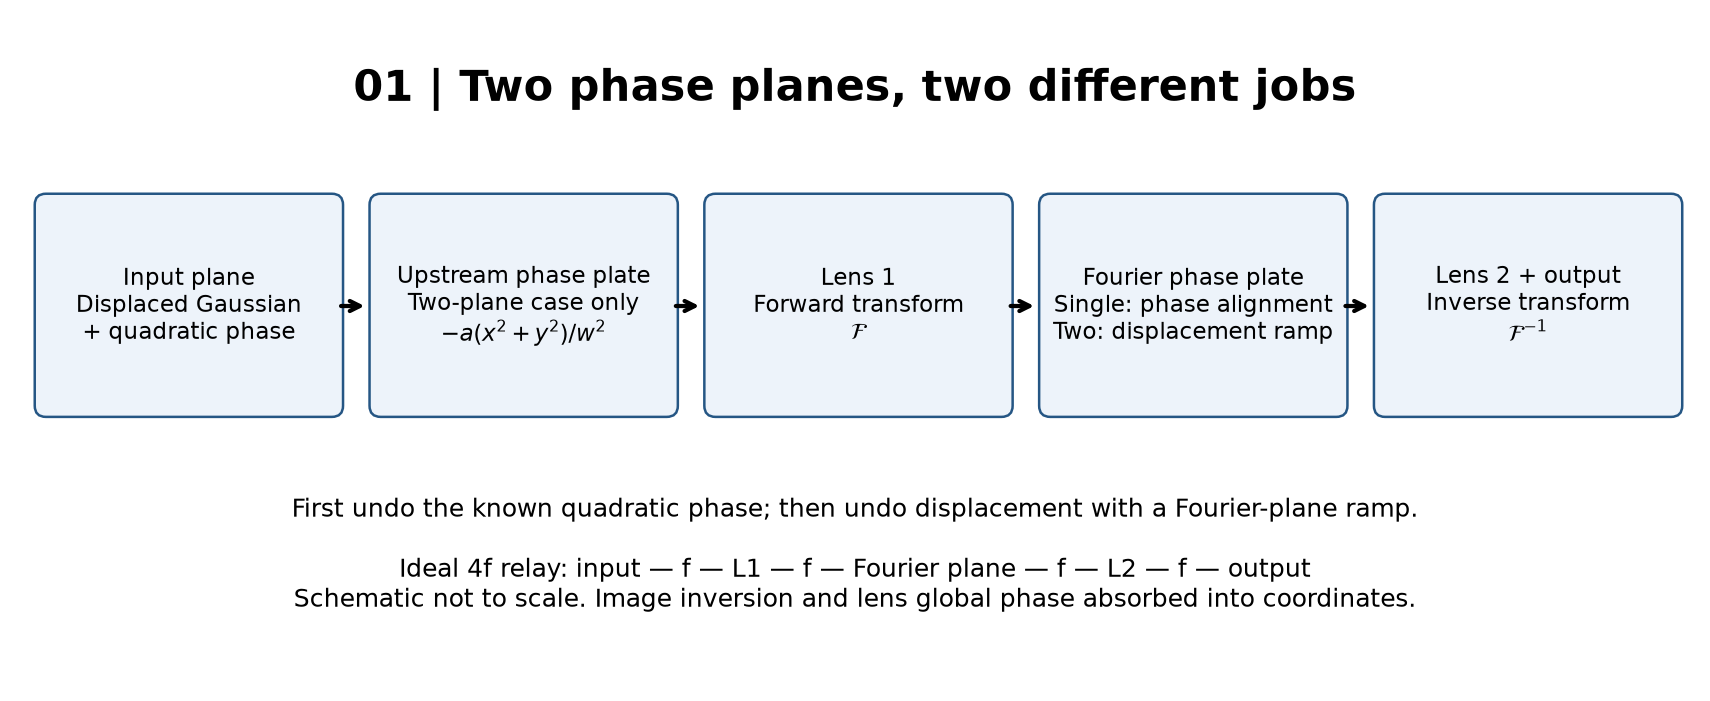
\includegraphics[width=\linewidth]{output/01_optical_schematic.png}
\caption{Conceptual ordering of the ideal relay, not to scale. The upstream plate is present only in the two-plane case. With one plane, the Fourier mask aligns the input spectrum's phase with the target. With two planes, the upstream plate first removes quadratic phase and the Fourier plate then removes displacement. The lower annotation gives the focal-length spacings.}
\label{fig:layout}
\end{figure}

\newpage
\section{Fields, overlap, and the displacement correction}
Write $\rvec=(x,y)$ and $\dvec=(d_x,d_y)$. The target and displaced fields are
\begin{equation}
 u_0(\rvec)=C e^{-|\rvec|^2/w^2},\qquad
 u_d(\rvec)=C_d e^{-|\rvec-\dvec|^2/w^2}.
\end{equation}
The constants normalize integrated power to one. The waist $w$ is the field's $1/e$ radius, or the intensity's $1/e^2$ radius. On an infinite plane $C_d=C$; the code normalizes the sampled fields separately. Window tails are negligible here.

For any candidate output $v$, define its normalized power overlap with the target as
\begin{equation}\label{eq:eta}
 \eta(v)=\frac{\left|\int u_0^*(\rvec)v(\rvec)\,\dd^2r\right|^2}{P_0P_v},
 \qquad P_v=\int |v|^2\,\dd^2r.
\end{equation}
This is a classical spatial-mode power fraction, not the unsquared amplitude overlap or a quantum fidelity. It equals one when the fields are proportional, allowing a constant global phase. Matching intensity images alone is not sufficient: a spatially varying phase can lower the overlap.

Use spatial frequencies $\fvec=(\nu_x,\nu_y)$ in cycles per metre, with the explicit sign convention
\begin{equation}\label{eq:FT}
 \widetilde u(\fvec)=\F[u]=\int u(\rvec)e^{-i2\pi\fvec\cdot\rvec}\,\dd^2r.
\end{equation}
Substitute $\mathbf s=\rvec-\dvec$ into this integral. The factor depending on displacement comes outside, giving the shift theorem and its compensating phase:
\begin{equation}\label{eq:shift}
 \widetilde u_d=\widetilde u_0 e^{-i2\pi\fvec\cdot\dvec},
 \qquad \boxed{\phi_{\rm shift}=+2\pi\fvec\cdot\dvec.}
\end{equation}
Thus $\F^{-1}[e^{i\phi_{\rm shift}}\widetilde u_d]=u_0$. The mask sign is \emph{positive} because the forward transform uses a negative exponent. A negative ramp would add displacement rather than cancel it. This works because displacement changes spectral phase but leaves spectral amplitude unchanged.
\begin{figure}[H]
\centering
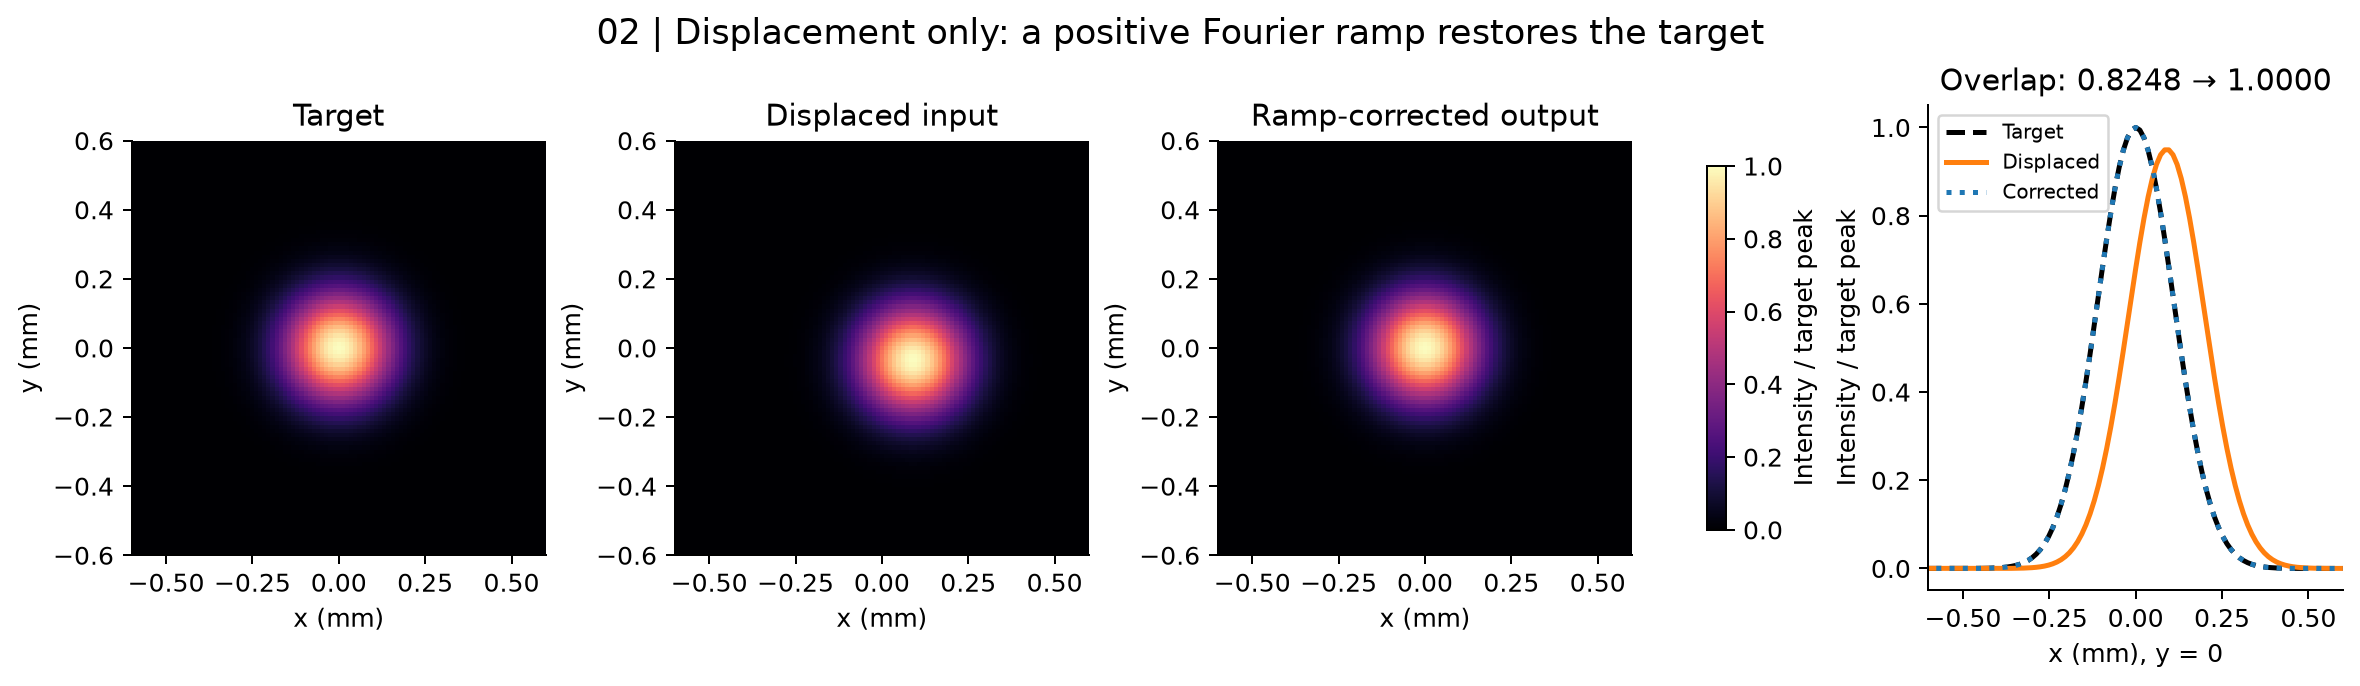
\includegraphics[width=\linewidth]{output/02_displacement_only.png}
\caption{Displacement alone. The first three panels show target, displaced, and ramp-corrected intensities on the same target-peak scale; axes are real-space millimetres. The last panel is a $y=0$ intensity section: target black dashed, displaced orange solid, corrected blue dotted. Target and corrected curves coincide. The full two-dimensional power overlap improves from 0.824758 to 1; complex-field recovery is checked separately.}
\label{fig:shift}
\end{figure}
The displacement is sampled as a continuous Gaussian with a fractional-pixel offset, not rounded to an integer shift. Figure~\ref{fig:shift} is therefore also a useful numerical test of the transform convention.

\newpage
\section{Why the best single Fourier plate has a ceiling}
Now add the known quadratic phase
\begin{equation}\label{eq:aberrated}
 u_a(\rvec)=u_d(\rvec)\exp\!\left(i a\frac{|\rvec|^2}{w^2}\right).
\end{equation}
Here $a$ is the dimensionless defocus coefficient (a phase in radians at radius $w$), not a propagation distance. This phase is centered on the \textbf{optical axis}, not on the displaced beam. With $\rvec=\mathbf s+\dvec$, its argument contains
\begin{equation}
 a\frac{|\rvec|^2}{w^2}=a\frac{|\mathbf s|^2}{w^2}
 +\frac{2a}{w^2}\mathbf s\cdot\dvec+a\frac{|\dvec|^2}{w^2}.
\end{equation}
The middle term is linear across the beam. Consequently, even without an independently imposed tilt, the spectrum both broadens and shifts. Treating this as only centered spectral broadening would describe a different input.

For a fixed input spectrum $A=\widetilde u_a$ and target spectrum $T=\widetilde u_0$, Parseval's identity lets us evaluate the overlap in Fourier space. A mask multiplies $A$ by $e^{i\phi}$, so $|Ae^{i\phi}|=|A|$ at every frequency. The triangle inequality gives
\begin{equation}\label{eq:bound}
 \eta\leq \eta_{\rm max}^{(1)}=
 \frac{\left(\int |T|\,|A|\,\dd^2\nu\right)^2}{P_0P_a}.
\end{equation}
This is an attainable ceiling, not just an estimate. Choose
\begin{equation}\label{eq:best}
 \boxed{\phi_{\rm best}=\arg(TA^*)=\arg T-\arg A\pmod{2\pi}.}
\end{equation}
Then every term in $T^*Ae^{i\phi_{\rm best}}$ is real and nonnegative, attaining equality in the triangle inequality. At zeros, the phase is arbitrary. Cauchy--Schwarz further implies $\eta_{\rm max}^{(1)}\leq1$, with equality only when $|A|$ and $|T|$ are proportional almost everywhere. The best phase cannot remove an amplitude mismatch. Equation~\eqref{eq:best} is calculated directly from the known fields; it is not a trained mask and is more general than a displacement ramp.
\begin{figure}[H]
\centering
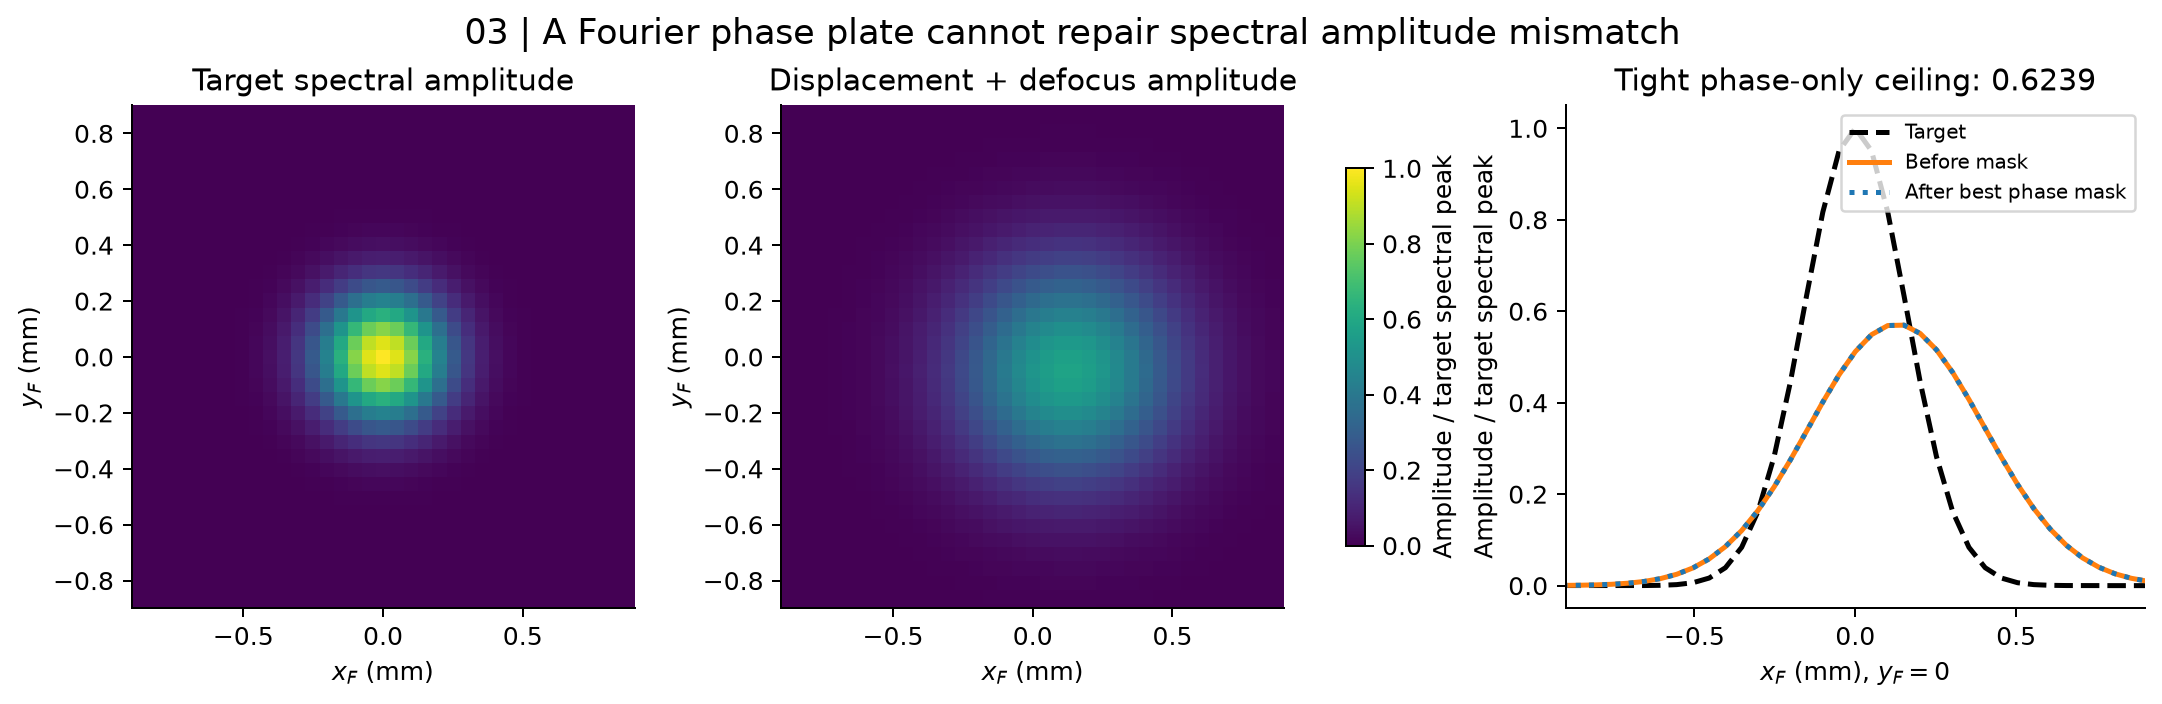
\includegraphics[width=\linewidth]{output/03_spectral_amplitude_limit.png}
\caption{Spectral \emph{amplitude}, not intensity, in physical Fourier-plane millimetres. The maps show target and aberrated amplitudes, normalized to the target spectral peak. The $y_F=0$ slice compares target (black dashed), before correction (orange solid), and after best phase correction (blue dotted). Before and after coincide: the mask cannot change spectral amplitude. The 0.623926 ceiling uses the entire two-dimensional plane, not just this slice.}
\label{fig:amplitude}
\end{figure}

\newpage
\section{Two separated planes: cancel phase, then recenter}
For this particular known distortion, the remedy is elementary. Put the opposite quadratic phase at the input plane:
\begin{equation}\label{eq:up}
 \boxed{\phi_{\rm up}(\rvec)=-a|\rvec|^2/w^2.}\qquad
 u_a e^{i\phi_{\rm up}}=u_d.
\end{equation}
The negative sign cancels the positive phase in Eq.~\eqref{eq:aberrated} point by point, about the same optical axis. The Fourier-plane positive ramp from Eq.~\eqref{eq:shift} then cancels displacement:
\begin{equation}\label{eq:two}
 v_2=\F^{-1}\!\left[e^{i\phi_{\rm shift}}
 \F\!\left[u_a e^{i\phi_{\rm up}}\right]\right]=u_0.
\end{equation}
Both elements are phase-only and preserve power. Nevertheless, the upstream element changes the spectrum \emph{arriving} at the Fourier plane. The bound in Eq.~\eqref{eq:bound} assumed that incident spectrum was fixed, so there is no contradiction. Two plates placed in the \emph{same} Fourier plane would merely add their phases and retain the same amplitude limitation.
\begin{figure}[H]
\centering
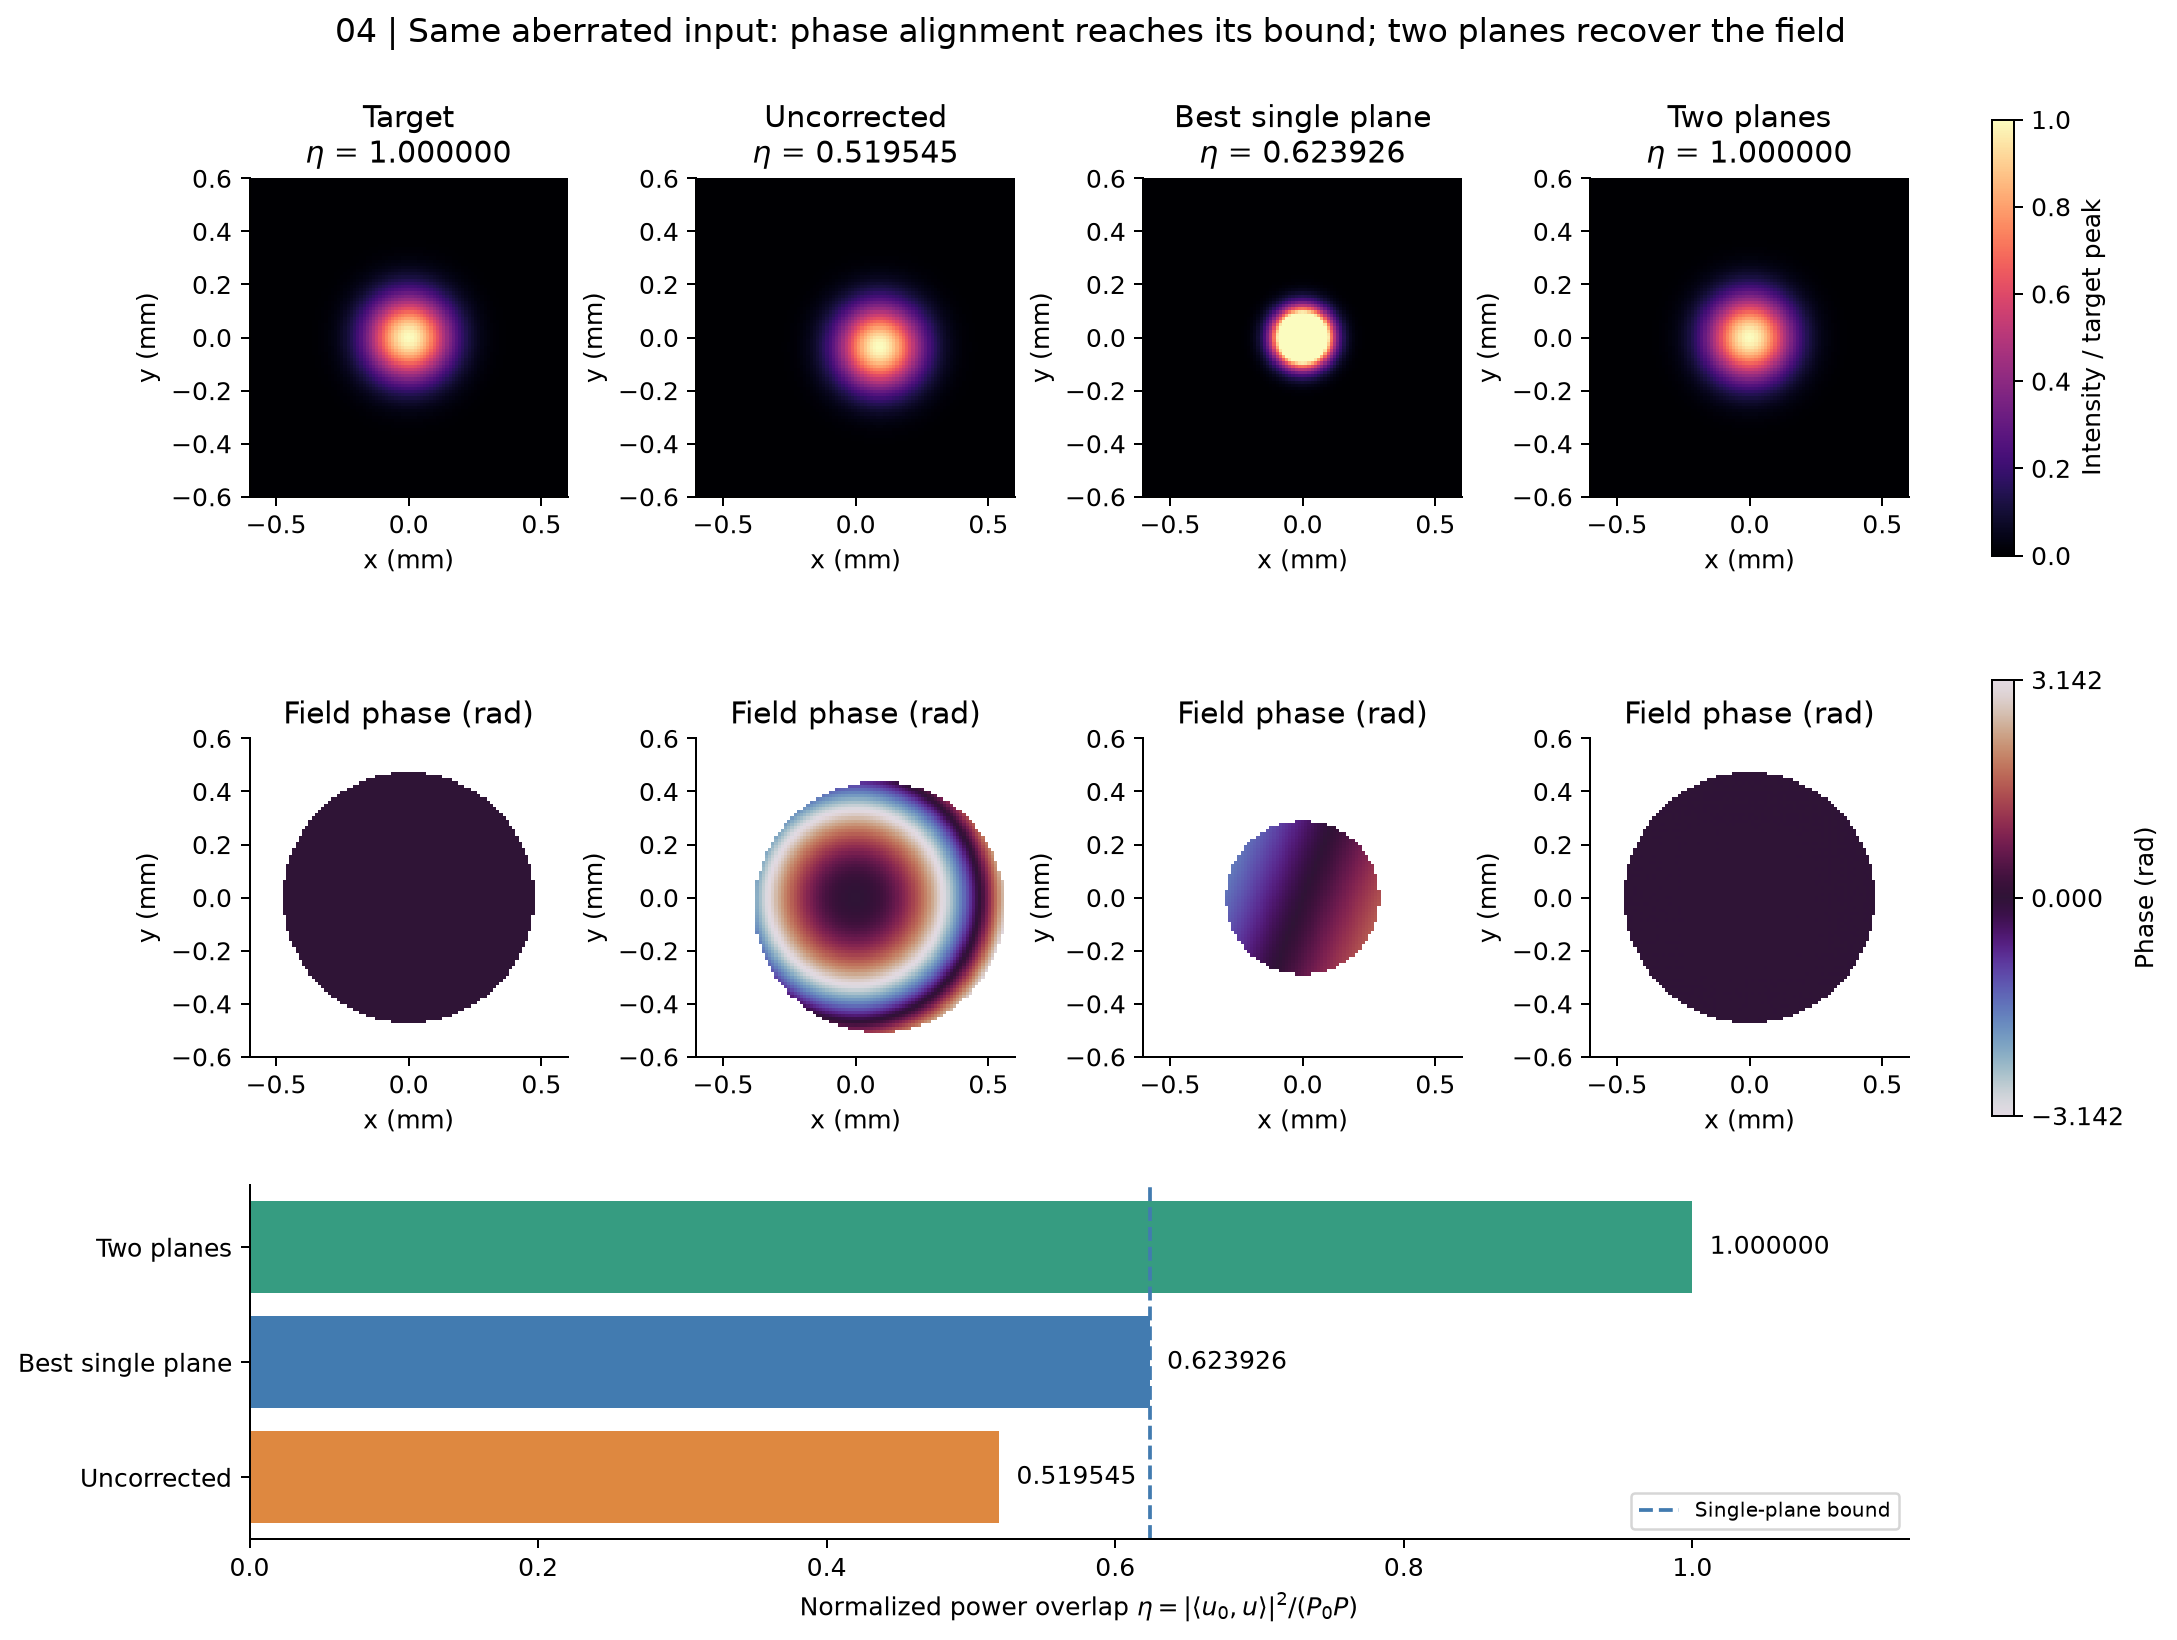
\includegraphics[width=0.94\linewidth]{output/04_correction_comparison.png}
\caption{Same displacement-plus-defocus input throughout. Columns show target, uncorrected, best single-plane correction, and two-plane correction. Top: intensity on a common target-peak scale. Middle: field phase in radians from $-\pi$ to $\pi$, hidden below $10^{-4}$ of the target peak intensity. Both rows use real-space millimetres. Bottom: full-field power overlaps, with the single-plane ceiling dashed. Phase alignment reaches its ceiling; two separated planes recover the target field to numerical precision.}
\label{fig:comparison}
\end{figure}
Equation~\eqref{eq:two} proves recovery only for the specified displacement-plus-quadratic-phase family with exactly known parameters. It is not a universal theorem that two phase plates correct every possible field.

\newpage
\section{Numerical experiment and independent checks}
\subsection{Parameters and physical normalization}
The standalone implementation is \texttt{run\_demo.py}, using NumPy and Matplotlib. There is one deterministic input per case, no random jitter, no parameter fitting, and no optimizer. The wavelength is $1550\,$nm, focal length $f=100\,$mm, waist $w=220\,\mu$m, displacement $(d_x,d_y)=(90,-35)\,\mu$m, and defocus coefficient $a=1.4$. There is no imposed tilt or astigmatism.

A $256\times256$ grid has pitch $\Delta x=12\,\mu$m and width $3.072\,$mm. The grid is larger than the research model's $128\times128$ grid to suppress finite-window tails. The FFT has periodic boundaries, but the Gaussian tails are negligible at the boundaries in this example. Display crops do not limit the calculation: field images show $\pm0.6\,$mm and spectral images show $\pm0.9\,$mm, while overlap uses the full arrays.

Let $\F_d$ be the centered, orthonormal array FFT. Frequency maps to the physical focal plane by $x_F=\lambda f\nu_x$, and similarly for $y_F$. Its sample pitch and physical field are
\begin{equation}
 \Delta x_F=\frac{\lambda f}{N\Delta x},\qquad
 U_F=\frac{\Delta x}{\Delta x_F}\F_d u,\qquad
 \sum |U_F|^2\Delta x_F^2=\sum |u|^2\Delta x^2.
\end{equation}
The scaling matters when labeling Fourier-plane amplitude and checking physical power. Forward and inverse factors cancel in the relay, so unitary array FFTs can implement the masks directly. The same overlap bound follows in either frequency or physical focal-plane coordinates with consistent measures.

\subsection{Saved results and continuum predictions}
Table~\ref{tab:results} reports the new reference run in \texttt{output/metrics.json}. All entries refer to nominal fixed fields, not means over a test ensemble.
\begin{table}[H]
\centering
\caption{Normalized power overlap for the deterministic classroom model.}
\label{tab:results}
\begin{tabular}{llr}
\toprule
Input & Correction & $\eta$ \\
\midrule
Displacement & None & 0.824758 \\
Displacement & Positive Fourier ramp & 1.000000 \\
Displacement + defocus & None & 0.519545 \\
Displacement + defocus & Best single Fourier plane & 0.623926 \\
Displacement + defocus & Input plate + Fourier ramp & 1.000000 \\
\bottomrule
\end{tabular}
\end{table}
For an independent infinite-plane check, define $D=|\dvec|^2/w^2$. Gaussian integration gives
\begin{align}
 \eta(u_d)&=e^{-D},\\
 \eta(u_a)&=\frac{\exp[-D(1+a^2/(4+a^2))]}{1+a^2/4},\\
 \eta_{\rm max}^{(1)}&=\frac{4(1+a^2)}{(2+a^2)^2}
 \exp\!\left[-\frac{2a^2D}{2+a^2}\right].\label{eq:analyticbound}
\end{align}
These expressions can be obtained by completing the square in the Gaussian integrals. In particular, $|\widetilde u_a|$ has width broadened by $\sqrt{1+a^2}$ and center $\fvec_c=a\dvec/(\pi w^2)$. Integrating its product with $|\widetilde u_0|$ gives Eq.~\eqref{eq:analyticbound}. The displacement-dependent exponential must remain because the defocus is axis-centered.

\newpage
\section{What the checks establish---and what they do not}
The saved numerical values agree with the independent continuum expressions to a maximum absolute difference of $6.66\times10^{-16}$. The directly computed spectral-amplitude ceiling is 0.6239259445257388, while the phase-aligned output gives 0.6239259445257396. The difference is floating-point rounding, not a physical violation of the bound.

The relative complex-field error $\|v-u_0\|_2/\|u_0\|_2$ is $4.25\times10^{-16}$ after displacement correction and $4.45\times10^{-16}$ after two-plane correction. These checks are stronger than comparing intensity plots: they test both amplitude and phase. Spatial and physically scaled Fourier powers remain one to rounding error. The reported unit overlaps are not obtained by clipping the computed metric to the interval $[0,1]$.

The accompanying demo test suite checks power and Parseval consistency, inverse FFT recovery, the fractional shift theorem and a wrong-sign negative control, attainment of the phase-only bound, preservation of spectral amplitude, and two-plane complex-field recovery. It also compares the continuum formulas and a $512\times512$, $6\,\mu$m resolution cross-check, and checks output names and saved arrays. The resolution comparison is a numerical consistency test, not a statistical sweep. The demo README and its verification log describe these tests; the manuscript does not require retraining or regenerating archived figures.

\subsection{Interpretation and practical limits}
The result $\eta=1$ means ideal nominal numerical recovery under this model. Real phase plates have finite apertures, finite pixels, limited phase resolution, and calibration errors. Unknown or fluctuating displacement and defocus would make the prescribed cancellation imperfect. None of those effects is measured or modeled here. Nor does removing the pupil imply that a real lens has infinite clear aperture; it is a deliberate simplification that removes one loss mechanism from the question.

A lossless phase correction can redistribute power among modes without creating power. The improvement from 0.519545 to 0.623926 is therefore better target-mode matching, not amplification. The remaining mismatch is not evidence that the best mask was trained poorly: no training occurs, and the phase-alignment solution attains the fixed-input ceiling. To go beyond that ceiling, the allowed optical operations must change, as the upstream plate does here.

\subsection{Optional research extensions, not prerequisites}
The larger research manuscript, \href{../paper/main.pdf}{\texttt{../paper/main.pdf}}, studies additional distortions, jittered ensembles, optimization, and a receiver model. Those are possible extensions after the present Fourier-optics argument is understood. Its historical approximately $0.45\to0.95$ ensemble comparison belongs to a different, fluctuating-input study; it must not be substituted for the deterministic values in Table~\ref{tab:results}. The original research manuscript and its evidence are preserved separately.

Training could be investigated when a mask must serve uncertain inputs, but it cannot evade the fixed-input spectral-amplitude constraint of one Fourier plane. A quantum or coherent-receiver extension would require additional assumptions about states, detection, and noise. The present classical overlap calculation alone establishes neither a quantum-noise advantage nor a communication-security result.

\section{Conclusion}
The shift theorem identifies the correct positive Fourier ramp for displacement. Quadratic phase about the optical axis changes spectral amplitude as well as phase, so a single Fourier plate cannot generally restore the target. Aligning spectral phases yields the exact attainable overlap ceiling, 0.623926 for the chosen combined distortion. An upstream negative quadratic phase followed by the positive Fourier ramp recovers the known nominal field to numerical precision. The lesson is a distinction between optical capabilities: correcting phase at one fixed spectrum is not the same as changing the spectrum that reaches that plane.

\end{document}
